\documentclass[landscape,20pt]{foils}

% Packages
\usepackage[utf8]{inputenc}
\usepackage[T1]{fontenc}
\usepackage{helvet}
\renewcommand{\familydefault}{\sfdefault}

\usepackage[landscape,margin=0.5in]{geometry}
\usepackage[table]{xcolor}
\usepackage{graphicx}
\usepackage{amsmath,amssymb}
\usepackage{booktabs}
\usepackage{tabularx}
\usepackage{array}
\usepackage{enumitem}
\usepackage{tikz}
\usetikzlibrary{positioning,calc,shapes.geometric,backgrounds,patterns,arrows.meta}
\usepackage[most]{tcolorbox}
\usepackage{fontawesome5}

% Custom Color Palette (Deep Slate & Vibrant Accents)
\definecolor{NavyDark}{RGB}{15,23,42}
\definecolor{TealAccent}{RGB}{14,165,233}
\definecolor{IndigoAccent}{RGB}{99,102,241}
\definecolor{EmeraldAccent}{RGB}{16,185,129}
\definecolor{SlateText}{RGB}{51,65,85}
\definecolor{SlateLightText}{RGB}{100,116,139}
\definecolor{LightBg}{RGB}{248,250,252}
\definecolor{CardBg}{RGB}{255,255,255}
\definecolor{BorderColor}{RGB}{226,232,240}
\definecolor{TableAltBg}{RGB}{241,245,249}

% FoilTeX Header / Footer Setup
\MyLogo{\textcolor{SlateLightText}{\small \faBuilding\ Vertex Enterprise Systems \quad|\quad Annual Technology Summit 2026}}
\rightfooter{\textcolor{SlateLightText}{\small Slide \thepage}}
\leftheader{}
\rightheader{}

% List Styling
\setlist[itemize]{label=\textcolor{TealAccent}{\small\faAngleRight},leftmargin=*,itemsep=2pt,topsep=2pt}
\setlist[enumerate]{label=\textcolor{IndigoAccent}{\bfseries\arabic*.},leftmargin=*,itemsep=2pt,topsep=2pt}

% Custom tcolorbox Styles
\tcbset{
  slidecard/.style={
    enhanced,
    colback=CardBg,
    colframe=BorderColor,
    boxrule=1.5pt,
    arc=6pt,
    left=10pt, right=10pt, top=8pt, bottom=8pt,
    fonttitle=\bfseries\color{NavyDark},
    coltitle=NavyDark,
  },
  accentcard/.style={
    enhanced,
    colback=LightBg,
    colframe=TealAccent,
    boxrule=1.5pt,
    arc=6pt,
    left=10pt, right=10pt, top=8pt, bottom=8pt,
  },
  darkcard/.style={
    enhanced,
    colback=NavyDark,
    colframe=NavyDark,
    colupper=white,
    collower=white,
    arc=6pt,
    left=12pt, right=12pt, top=12pt, bottom=12pt,
  }
}

\begin{document}

% SLIDE 1: Title Slide
\begin{tcolorbox}[darkcard, height=0.80\textheight, halign=center, valign=center]
  \vspace{2pt}
  {\Huge \bfseries \textcolor{TealAccent}{VERTEX SYSTEMS}} \\[10pt]
  {\Huge \bfseries Next-Generation Cloud Infrastructure} \\[12pt]
  {\Large Scaling Distributed Enterprise Architectures for High-Throughput Workloads} \\[18pt]
  \tikz \draw[TealAccent, line width=2.5pt] (0,0) -- (10,0); \\[18pt]
  {\large \faUser\ Dr. Elena Rostova \quad|\quad Chief Technology Officer} \\[6pt]
  {\small \faGlobe\ Vertex Distributed Systems \quad\textbullet\quad \faCalendar\ October 2026}
\end{tcolorbox}

% SLIDE 2: Agenda
\foilhead{\textcolor{NavyDark}{\faListUl\ Presentation Agenda}}
\vspace{2pt}
\begin{minipage}[t]{0.48\textwidth}
  \begin{tcolorbox}[slidecard, title=\Large \faLayerGroup\ Technical Foundations]
    \begin{itemize}
      \item System Architecture Overview
      \item Distributed Consensus Engine
      \item High-Throughput Stream Processing
      \item Fault Tolerance \& Auto-Healing
    \end{itemize}
  \end{tcolorbox}
\end{minipage}%
\hfill
\begin{minipage}[t]{0.48\textwidth}
  \begin{tcolorbox}[slidecard, title=\Large \faLock\ Security \& Operations]
    \begin{itemize}
      \item Zero-Trust Security Framework
      \item Performance Benchmarks \& SLA
      \item Enterprise Deployment Strategy
      \item 2027 Strategic Technology Roadmap
    \end{itemize}
  \end{tcolorbox}
\end{minipage}

% SLIDE 3: Section 1
\foilhead{}
\begin{tcolorbox}[darkcard, height=0.80\textheight, halign=center, valign=center]
  {\Huge \textcolor{TealAccent}{PART I}} \\[14pt]
  {\Huge \bfseries Architecture \& Core Principles} \\[12pt]
  {\Large Designing for Elasticity, Security, and Sub-Millisecond Latency}
\end{tcolorbox}

% SLIDE 4: Core Pillars
\foilhead{\textcolor{NavyDark}{\faCogs\ Core Architectural Pillars}}
\vspace{2pt}
\begin{minipage}[t]{0.31\textwidth}
  \begin{tcolorbox}[slidecard, title=\large \faServer\ Elastic Compute]
    Dynamic pod autoscaling with predictive workload provisioning.
    \begin{itemize}
      \item Multi-region clusters
      \item Sub-50ms cold starts
      \item Automated failover
    \end{itemize}
  \end{tcolorbox}
\end{minipage}%
\hfill
\begin{minipage}[t]{0.31\textwidth}
  \begin{tcolorbox}[slidecard, title=\large \faDatabase\ Storage Mesh]
    Distributed transactional storage engine built on Raft consensus.
    \begin{itemize}
      \item ACID compliance
      \item Multi-active replication
      \item Zero data loss (RPO=0)
    \end{itemize}
  \end{tcolorbox}
\end{minipage}%
\hfill
\begin{minipage}[t]{0.31\textwidth}
  \begin{tcolorbox}[slidecard, title=\large \faNetworkWired\ Event Highway]
    Real-time event streaming processing 10M+ events per second.
    \begin{itemize}
      \item Low-latency messaging
      \item Exactly-once delivery
      \item Native schema registry
    \end{itemize}
  \end{tcolorbox}
\end{minipage}

% SLIDE 5: Stream Processing
\foilhead{\textcolor{NavyDark}{\faChartLine\ High-Throughput Stream Processing}}
\vspace{2pt}
\begin{minipage}[t]{0.54\textwidth}
  \small
  Our stream processing framework ingests logs, metrics, and state transitions into a unified analytical layer.
  
  \begin{itemize}
    \item \textbf{Ingestion Layer:} Distributed Kafka brokers receiving encrypted telemetry.
    \item \textbf{Stream Engine:} Stateful vectorized memory execution.
    \item \textbf{Analytical Store:} Real-time columnar database supporting millisecond queries.
  \end{itemize}
\end{minipage}%
\hfill
\begin{minipage}[t]{0.42\textwidth}
  \begin{tcolorbox}[accentcard, title=\large \faBolt\ Measured Performance]
    \centering
    {\Large \bfseries \textcolor{IndigoAccent}{10.4M}} \\[2pt]
    {\small Events Processed per Second} \\[4pt]
    \tikz \draw[BorderColor, line width=1pt] (0,0) -- (4,0); \\[4pt]
    {\Large \bfseries \textcolor{EmeraldAccent}{2.4 ms}} \\[2pt]
    {\small P99 End-to-End Latency}
  \end{tcolorbox}
\end{minipage}

% SLIDE 6: TikZ Topology Diagram
\foilhead{\textcolor{NavyDark}{\faProjectDiagram\ End-to-End System Topology}}
\vspace{2pt}
\centering
\begin{tikzpicture}[scale=0.58, transform shape,
  box/.style={draw=NavyDark, fill=LightBg, line width=1.5pt, rounded corners=6pt, minimum width=3.4cm, minimum height=1.6cm, align=center, font=\bfseries\small},
  accentbox/.style={draw=TealAccent, fill=TealAccent!12, line width=1.5pt, rounded corners=6pt, minimum width=3.4cm, minimum height=1.6cm, align=center, font=\bfseries\small},
  darkbox/.style={draw=NavyDark, fill=NavyDark, text=white, line width=1.5pt, rounded corners=6pt, minimum width=3.4cm, minimum height=1.6cm, align=center, font=\bfseries\small},
  arrow/.style={->, >=stealth, line width=2pt, TealAccent}
]
  % Nodes
  \node[box] (client) {\faDesktop\ Edge Clients\\ (Web / Mobile / IoT)};
  \node[accentbox, right=1.6cm of client] (gateway) {\faGlobe\ API Gateway\\ (Envoy / OAuth2)};
  \node[darkbox, right=1.6cm of gateway] (services) {\faBoxes\ Microservices\\ (Go / Rust Core)};
  \node[accentbox, right=1.6cm of services] (db) {\faDatabase\ Distributed DB\\ (Vertex Storage)};

  % Flow arrows
  \draw[arrow] (client) -- node[above, font=\tiny\bfseries, text=SlateText] {gRPC / TLS} (gateway);
  \draw[arrow] (gateway) -- node[above, font=\tiny\bfseries, text=SlateText] {mTLS Auth} (services);
  \draw[arrow] (services) -- node[above, font=\tiny\bfseries, text=SlateText] {Read / Write} (db);

  % Lower queue node
  \node[box, below=1.2cm of services] (queue) {\faStream\ Event Queue\\ (Kafka Engine)};
  \draw[arrow] (services) -- node[right, font=\tiny\bfseries, text=SlateText] {Events} (queue);
  \draw[arrow] (queue) -| node[below, font=\tiny\bfseries, text=SlateText] {Async Processing} (db);
\end{tikzpicture}

% SLIDE 7: Section 2
\foilhead{}
\begin{tcolorbox}[darkcard, height=0.80\textheight, halign=center, valign=center]
  {\Huge \textcolor{TealAccent}{PART II}} \\[14pt]
  {\Huge \bfseries Performance \& Reliability} \\[12pt]
  {\Large Industry Benchmarks and High-Availability Engineering}
\end{tcolorbox}

% SLIDE 8: Table
\foilhead{\textcolor{NavyDark}{\faTable\ System Performance Comparison}}
\vspace{2pt}
\centering
\small
\renewcommand{\arraystretch}{1.2}
\rowcolors{2}{TableAltBg}{white}
\begin{tabularx}{\textwidth}{X c c c}
  \toprule
  \textbf{Performance Metric} & \textbf{Legacy Stack} & \textbf{Competitor Gen-3} & \textbf{Vertex System (New)} \\
  \midrule
  P95 Query Latency & 145 ms & 42 ms & \textbf{8.5 ms} \\
  P99 Ingestion Latency & 820 ms & 180 ms & \textbf{24 ms} \\
  Throughput Limit & 250k req/sec & 2.1M req/sec & \textbf{10.4M req/sec} \\
  Failover Recovery Time & 4.5 minutes & 30 seconds & \textbf{$<$ 1.2 seconds} \\
  Infrastructure Cost / 1M Req & \$0.42 & \$0.18 & \textbf{\$0.04} \\
  \bottomrule
\end{tabularx}

% SLIDE 9: High Availability
\foilhead{\textcolor{NavyDark}{\faCheck\ Fault Tolerance \& High Availability}}
\vspace{2pt}
\begin{minipage}[t]{0.48\textwidth}
  \begin{tcolorbox}[slidecard, title=\large \faServer\ Active-Active Replication]
    \begin{itemize}
      \item Synchronous multi-region consensus via Raft protocol.
      \item Zero single point of failure across compute nodes.
      \item Real-time state synchronization under high jitter.
    \end{itemize}
  \end{tcolorbox}
\end{minipage}%
\hfill
\begin{minipage}[t]{0.48\textwidth}
  \begin{tcolorbox}[slidecard, title=\large \faCogs\ Self-Healing Infrastructure]
    \begin{itemize}
      \item Automatic node isolation upon health check failure.
      \item Instant cluster re-balancing without manual intervention.
      \item Automated point-in-time state recovery.
    \end{itemize}
  \end{tcolorbox}
\end{minipage}

% SLIDE 10: Section 3
\foilhead{}
\begin{tcolorbox}[darkcard, height=0.80\textheight, halign=center, valign=center]
  {\Huge \textcolor{TealAccent}{PART III}} \\[14pt]
  {\Huge \bfseries Security, Compliance \& Governance} \\[12pt]
  {\Large Zero-Trust Architecture for Enterprise Data Protection}
\end{tcolorbox}

% SLIDE 11: Security
\foilhead{\textcolor{NavyDark}{\faLock\ Zero-Trust Security Architecture}}
\vspace{2pt}
\begin{minipage}[t]{0.48\textwidth}
  \begin{tcolorbox}[slidecard, title=\large \faKey\ Identity \& Access Management]
    \begin{itemize}
      \item Short-lived mTLS client certificate authentication.
      \item Role-Based Access Control (RBAC) fine-grained scopes.
      \item Continuous automated token rotation and verification.
    \end{itemize}
  \end{tcolorbox}
\end{minipage}%
\hfill
\begin{minipage}[t]{0.48\textwidth}
  \begin{tcolorbox}[slidecard, title=\large \faLock\ Data Protection \& Encryption]
    \begin{itemize}
      \item AES-256-GCM encryption at rest across all disks.
      \item TLS 1.3 in-transit encryption with Perfect Forward Secrecy.
      \item HSM-backed root key management and audit trails.
    \end{itemize}
  \end{tcolorbox}
\end{minipage}

% SLIDE 12: Section 4
\foilhead{}
\begin{tcolorbox}[darkcard, height=0.80\textheight, halign=center, valign=center]
  {\Huge \textcolor{TealAccent}{PART IV}} \\[14pt]
  {\Huge \bfseries Global Deployment \& Business Impact} \\[12pt]
  {\Large Multi-Phase Rollout and Measured Enterprise ROI}
\end{tcolorbox}

% SLIDE 13: Timeline
\foilhead{\textcolor{NavyDark}{\faTasks\ Global Rollout Timeline}}
\vspace{2pt}
\begin{minipage}[t]{0.48\textwidth}
  \begin{tcolorbox}[slidecard, title=\large Phase 1: Core Foundation (Q1 2026)]
    Deploy core control plane, IAM authentication service, and primary storage cluster in North America.
  \end{tcolorbox}
  \vspace{4pt}
  \begin{tcolorbox}[slidecard, title=\large Phase 2: Edge Expansion (Q2 2026)]
    Provision 14 edge caching pops across Europe and Asia-Pacific. Enable multi-region active-active routing.
  \end{tcolorbox}
\end{minipage}%
\hfill
\begin{minipage}[t]{0.48\textwidth}
  \begin{tcolorbox}[slidecard, title=\large Phase 3: Workload Migration (Q3 2026)]
    Seamless zero-downtime traffic cutover of enterprise telemetry workloads to Vertex platform.
  \end{tcolorbox}
  \vspace{4pt}
  \begin{tcolorbox}[slidecard, title=\large Phase 4: Full Autonomy (Q4 2026)]
    Enable automated ML-driven resource balancing and predictive scaling across all regional clusters.
  \end{tcolorbox}
\end{minipage}

% SLIDE 14: Metrics Cards
\foilhead{\textcolor{NavyDark}{\faChartBar\ Key Impact Metrics}}
\vspace{2pt}
\begin{minipage}[t]{0.23\textwidth}
  \begin{tcolorbox}[accentcard, halign=center]
    {\Large \bfseries \textcolor{NavyDark}{99.999\%}} \\[4pt]
    {\small System Uptime}
  \end{tcolorbox}
\end{minipage}%
\hfill
\begin{minipage}[t]{0.23\textwidth}
  \begin{tcolorbox}[accentcard, halign=center]
    {\Large \bfseries \textcolor{TealAccent}{65\%}} \\[4pt]
    {\small Cost Savings}
  \end{tcolorbox}
\end{minipage}%
\hfill
\begin{minipage}[t]{0.23\textwidth}
  \begin{tcolorbox}[accentcard, halign=center]
    {\Large \bfseries \textcolor{IndigoAccent}{12x}} \\[4pt]
    {\small Deploy Speed}
  \end{tcolorbox}
\end{minipage}%
\hfill
\begin{minipage}[t]{0.23\textwidth}
  \begin{tcolorbox}[accentcard, halign=center]
    {\Large \bfseries \textcolor{EmeraldAccent}{0 ms}} \\[4pt]
    {\small Data Loss (RPO)}
  \end{tcolorbox}
\end{minipage}

% SLIDE 15: Q&A / Closing
\foilhead{}
\begin{tcolorbox}[darkcard, height=0.80\textheight, halign=center, valign=center]
  {\Huge \textcolor{TealAccent}{\faComments}} \\[14pt]
  {\Huge \bfseries Questions \& Discussion} \\[18pt]
  {\Large Thank you for attending!} \\[20pt]
  \tikz \draw[TealAccent, line width=2.5pt] (0,0) -- (10,0); \\[20pt]
  {\large \faEnvelope\ contact@vertex-systems.example \quad|\quad \faGlobe\ https://vertex-systems.example} \\[8pt]
  {\small Documentation \& API Specifications available at developer.vertex-systems.example}
\end{tcolorbox}

\end{document}
